\documentclass[10pt]{beamer}

\newcommand{\lectnum}{L02}
\newcommand{\lecttitle}{Machine Learning Concepts}

\usepackage{amsmath, amssymb, graphicx}
\usepackage[]{algorithm2e}
\usepackage{pdfpages}
\usepackage[british]{babel}

\hypersetup{colorlinks,linkcolor=,urlcolor=blue}
\newenvironment{titledslide}[1]{\begin{frame}\frametitle{#1}}{\end{frame}}

\mode<presentation>{\setbeamercovered{transparent}}

\setbeamertemplate{sidebar right}{}
\setbeamertemplate{footline}{%
\hfill\usebeamertemplate***{navigation symbols}
\hspace{0.4cm}\lectnum: \insertframenumber{}/\inserttotalframenumber \hspace*{0.4cm}}

\author{James Cussens}

\title{COMS30035, Machine learning:\\ \vspace{5pt} \lecttitle}

\institute{School of Computer Science\\University of Bristol}

\begin{document}
%%%%%%%%%%%%%%%%%%%%%%%%%%%%%%%%%%%%%%%%%%%%%%%%%%%%%%%%%%%%%%%%%%%%%%

\begin{frame}
  \titlepage
\end{frame}

%%%%%%%%%%%%%%%%%%%%%%%%%%%%%%%%%%%%%%%%%%%%%%%%%%%%%%%%%%%%%%%%%%%%%%


%%%%%%%%%%%%%%%%%%%%%%%%%%%%%%%%%%%%%%%%%%%%%%%%%%%%%%%%%%%%%%%%%%%%%%
\begin{titledslide}{Acknowledgement}

  \begin{itemize}
  \item These slides are adapted from ones originally created by
    \href{https://www.dpag.ox.ac.uk/team/rui-ponte-costa}{Rui Ponte Costa}. 
  \end{itemize}
  
\end{titledslide}
%%%%%%%%%%%%%%%%%%%%%%%%%%%%%%%%%%%%%%%%%%%%%%%%%%%%%%%%%%%%%%%%%%%%%%
\begin{titledslide}{Textbooks}

  We will go over ML concepts following Chapter 1 of both textbooks:

  \begin{itemize}
  \item Bishop, C. M., Pattern recognition and machine learning
    (2006). Available for free \href{https://www.microsoft.com/en-us/research/people/cmbishop/prml-book/}{here}.	
\item Murphy, K., Probabilistic Machine Learning: An Introduction
  (2022). This book is also freely available \href{https://probml.github.io/pml-book}{here}.
\end{itemize}

\end{titledslide}
%%%%%%%%%%%%%%%%%%%%%%%%%%%%%%%%%%%%%%%%%%%%%%%%%%%%%%%%%%%%%%%%%%%%%% 
\begin{frame}[fragile]
\frametitle{Agenda}

\begin{itemize}
\item The different forms of machine learning:
  \begin{itemize}
  \item Unsupervised learning
  \item Supervised learning
  \item Reinforcement learning \vspace{10pt}
  \end{itemize}
\item Other important concepts in ML:
  \begin{itemize}
  \item Overfitting	
  \item Model selection
  \item The curse of dimensionality
  \item No free lunch theorem
  \item Parametric vs non-parametric models
  \end{itemize}
\end{itemize}

\end{frame}
%%%%%%%%%%%%%%%%%%%%%%%%%%%%%%%%%%%%%%%%%%%%%%%%%%%%%%%%%%%%%%%%%%%%%% 
\begin{frame}[fragile]

  \frametitle{The different forms of machine learning}
  \centerline{
\includegraphics[scale=0.2]{world_data.pdf}}
  \begin{itemize}
  \item ML attempts to learn \textbf{models} of the world
    \begin{itemize}
    \item Usually with many simplifications
    \item Models are a way of understanding how \textbf{input} data relates to the  \textbf{outputs}
    \item E.g., a function that maps weather observations to predictions
    \end{itemize}	
    % \item\uncover<2->{Models are simplifications of the world: }
    %   \uncover<3->{\begin{itemize}
    %   \item \textbf{``All models are wrong,  some are useful.''} -- George Box, 1976
    %   \end{itemize}}
  \end{itemize}
\end{frame}
%%%%%%%%%%%%%%%%%%%%%%%%%%%%%%%%%%%%%%%%%%%%%%%%%%%%%%%%%%%%%%%%%%%%%%
\begin{frame}[fragile]

  \frametitle{The different forms of machine learning}
  \centerline{
\includegraphics[scale=0.2]{world_data.pdf}}
  \begin{itemize}
  \item ML attempts to \textbf{learn} models of the world
    \begin{itemize}
    \item\uncover<2->{Many different flavours of data are available!
        \vspace{10pt}}
    \end{itemize}
  \uncover<3->{
  \item The data available defines which form of learning we can
    use\vspace{10pt}} \uncover<4->{
  \item However, the principle is always the same: \underline{model
      the data}..
    \begin{itemize}
    \item \dots the model assumptions and data structure vary
    \end{itemize}
  \end{itemize}}

\end{frame}
%%%%%%%%%%%%%%%%%%%%%%%%%%%%%%%%%%%%%%%%%%%%%%%%%%%%%%%%%%%%%%%%%%%%%%
\begin{frame}[fragile]

  \frametitle{Unsupervised learning}
  Only the input data is provided and models learn to extract patterns from the data.\vspace{5pt}
  \centerline{\includegraphics[scale=0.5]{unsupervised_learning.pdf}}
  
  \uncover<2->{
    Example tasks \footnote{Note that virtually all models that do not use explicit teaching signals, such as targets/labels or rewards are unsupervised.}:
    \begin{itemize}
    \item Clustering: grouping similar items together (e.g., K-means, unsupervised HMM) \vspace{3pt}
    \item Dimensionality reduction (e.g.\ PCA): finding a simplified representation of input data with fewer dimensions \vspace{3pt}
    \item Density estimation (mixture models,  language models):  used to estimate the probabilities of input data points \vspace{3pt}	
    \end{itemize}
  }
  
\end{frame}
%%%%%%%%%%%%%%%%%%%%%%%%%%%%%%%%%%%%%%%%%%%%%%%%%%%%%%%%%%%%%%%%%%%%%%
\begin{frame}[fragile]

  \frametitle{Supervised learning\vspace{3pt}}
  Each input is paired with an output -- a ``label'' or ``target'' -- and the model is trained to minimise the error (difference) between its output and the target.\vspace{5pt}
  \centerline{\includegraphics[scale=0.45]{supervised_learning.pdf}}
  
  \uncover<2->{
    Example tasks:
    \begin{itemize}
    \item Regression: numerical outputs (e.g.\  air temperatures over time)
    \item Classification: category labels (e.g.\  dog or bagel?) \vspace{3pt}
    \end{itemize}
  }
  \uncover<3->{
    Many learning methods can be used for both regression and classification:
    \begin{itemize}
    \item Supervised neural networks
    \item Support vector machines
    \item Decision trees
    \end{itemize}
  }
  
\end{frame}
%%%%%%%%%%%%%%%%%%%%%%%%%%%%%%%%%%%%%%%%%%%%%%%%%%%%%%%%%%%%%%%%%%%%%%
\begin{frame}[fragile]
  \frametitle{Reinforcement learning} The correct outputs are not
  given, but the model receives a reward (or punishment) depending on
  its actions.  \vspace{12pt}

  RL deals with dynamic environments where agents carry out sequences
  of actions.  It is inspired by animal behaviour. RL is seen as a
  field on its own -- \emph{we do \textbf{not} teach RL on this
    unit}.\vspace{5pt}
  \centerline{\includegraphics[scale=0.5]{reinforcement_learning.pdf}}

  \uncover<2->{ Examples:
    \begin{itemize}
    \item Temporal difference learning \vspace{3pt}
    \item Deep reinforcement learning (uses neural networks)
      \vspace{3pt}
    \end{itemize}
  }

\end{frame}
%%%%%%%%%%%%%%%%%%%%%%%%%%%%%%%%%%%%%%%%%%%%%%%%%%%%%%%%%%%%%%%%%%%%%%
\begin{frame}[fragile]

  \frametitle{Underfitting vs overfitting\vspace{3pt}}

  \underline{Underfitting}: A model that is too simple -- it should be
  as ``simple as possible, but no simpler.''\footnote{\begin{tiny}As
      Einstein used to say when formulating theories ``Everything
      should be made as simple as possible, but no
      simpler.''\end{tiny}}\\ \vspace{10pt}
  \uncover<4->{\underline{Overfitting}: A model that fits minor
    variations or noise; highly flexible models are particularly prone
    to overfitting.}\\ \vspace{5pt}


  \uncover<2->{Example from \emph{scikit-learn} \begin{small}(click
      \href{https://scikit-learn.org/stable/auto_examples/model_selection/plot_underfitting_overfitting.html}{here})\end{small}:}
  \centerline{\uncover<2->{\includegraphics[scale=0.28]{under_overfitting_1.png}
      \hspace{6pt}}
    \uncover<3->{\includegraphics[scale=0.28]{under_overfitting_2.png}
      \hspace{6pt}}
    \uncover<4->{\includegraphics[scale=0.28]{under_overfitting_3.png}}}

  % \centerline{\includegraphics[scale=0.3]{Figures2/Google_ML_trend-01.png}}
\end{frame}
%%%%%%%%%%%%%%%%%%%%%%%%%%%%%%%%%%%%%%%%%%%%%%%%%%%%%%%%%%%%%%%%%%%%%%
\begin{frame}[fragile]

  \frametitle{Model selection}

  There are an infinite number of models, how do we choose just one?
  Answer: We perform model selection to reduce
  under/overfitting.\footnote{Note that models that overfit or
    underfit fail to \textbf{generalise} to new data, this idea
    underlies model selection.}\\ \vspace{6pt}
  A common method is to \emph{split the dataset}. Lets look again at the data used in the previous slide\\
  \vspace{10pt}
  \centerline{\includegraphics[scale=0.5]{model_selection_1.png}}

\end{frame}
%%%%%%%%%%%%%%%%%%%%%%%%%%%%%%%%%%%%%%%%%%%%%%%%%%%%%%%%%%%%%%%%%%%%%%
\begin{frame}[fragile]

  \frametitle{Model selection} Lets split the full dataset
  into:\vspace{5pt}
\begin{itemize}
\item \textbf{Training dataset}: Used for training/optimising your
  model \begin{small}(e.g.\ use 80\% of the full dataset)\end{small}
\item \uncover<2->{\textbf{Validation dataset}: Used \emph{only} for
    validating your model \begin{small}(e.g.\ use 20\% of the full
      dataset)\end{small}}
\end{itemize}
\vspace{10pt}
\centerline{\includegraphics[scale=0.5]{model_selection_2.png} \hspace{6pt} \uncover<2->{\includegraphics[scale=0.5]{model_selection_3.png}}}

\end{frame}
%%%%%%%%%%%%%%%%%%%%%%%%%%%%%%%%%%%%%%%%%%%%%%%%%%%%%%%%%%%%%%%%%%%%%%
\begin{frame}[fragile]
  
  \frametitle{Model selection} Relying only on the validation dataset
  to select our models can lead us to overfit to that data, in
  particular for small datasets and iterative methods. So it is often
  common to use a third subset, the \emph{testing
    dataset}.\vspace{5pt}
  \begin{itemize}
  \item \textbf{Testing dataset}: Used to test the model for general
    fitting quality after the optimisation procedure has
    finished \begin{small}(e.g.\ use 10\% of the full
      dataset)\end{small}.
\end{itemize}
\vspace{10pt}
\centerline{\includegraphics[scale=0.5]{model_selection_4.png}}

\end{frame}
%%%%%%%%%%%%%%%%%%%%%%%%%%%%%%%%%%%%%%%%%%%%%%%%%%%%%%%%%%%%%%%%%%%%%%
\begin{frame}[fragile]

  \frametitle{Model selection} However, simply splitting the data
  means that we end up with less data for training the model. A
  solution is to cycle over multiple subsets of the data using
  \emph{cross-validation}.\vspace{5pt}
\begin{itemize}
\item \begin{small}\textbf{Cross-validation}: The original data is
    split into $S$ groups so that $(S-1)/S$ data is used for
    training. It is common to set $S$ to a relatively low number,
    e.g.\ $S=4$, which gives 4-fold cross validation using 3 (75\% of
    the data) subsets for training (white blocks) and 1 for validation
    (red block) for each run.\footnote{If $S=N$ where N is the full
      number of data samples it gives the \emph{leave-one-out}
      method.}\end{small}
\end{itemize}
\vspace{10pt}
\centerline{\includegraphics[scale=0.4]{cross_validation.png}}

\end{frame}
%%%%%%%%%%%%%%%%%%%%%%%%%%%%%%%%%%%%%%%%%%%%%%%%%%%%%%%%%%%%%%%%%%%%%%
\begin{frame}[fragile]

  \frametitle{Agenda}
  \begin{itemize}
  \item The different forms of machine learning:
    \begin{itemize}
    \item Unsupervised learning
    \item Supervised learning
    \item Reinforcement learning \vspace{10pt}
    \end{itemize}
  \item Other important concepts in ML:
    \begin{itemize}
    \item Overfitting	
    \item Model selection
    \item \textbf{The curse of dimensionality}
    \item \textbf{No free lunch theorem}
    \item \textbf{Parametric vs non-parametric models}
      % \item Decision theory (and information theory?)			
    \end{itemize}
  \end{itemize}

\end{frame}
%%%%%%%%%%%%%%%%%%%%%%%%%%%%%%%%%%%%%%%%%%%%%%%%%%%%%%%%%%%%%%%%%%%%%%
\begin{frame}[fragile]

  \frametitle{Curse of dimensionality in ML} 1D and 2D spaces can be
  covered by data easily, but for higher dimensions this is no longer
  feasible.
  \begin{itemize}
  \item \begin{small}If we were to divide the space into cells we
      would quickly need an exponentially large quantity of data to
      fill in all cells (see schematic below).\end{small}
    \uncover<2->{\item However, its often possible to find effective
      algorithms for two reasons (Bishop book):
      \begin{itemize}
      \item Data is often restricted to specific regions of the much
        bigger spaces -- i.e.\ effective dimensionality is much
        smaller.
      \item Data typically has smoothness properties -- i.e.\ small
        changes in the input variables will lead to small changes in
        the output variables.
      \end{itemize}}
  \end{itemize}
  \centerline{\includegraphics[scale=0.15]{curve_dim.png}}

\end{frame}
%%%%%%%%%%%%%%%%%%%%%%%%%%%%%%%%%%%%%%%%%%%%%%%%%%%%%%%%%%%%%%%%%%%%%%
\begin{frame}[fragile]
\frametitle{No free lunch theorem}
\emph{All models are wrong, but some models are useful. --- George Box 1976}\\\vspace{10pt}

\uncover<2->{\begin{itemize}
	\item Using model selection we can obtain a \emph{good model}.
	\item \emph{But} there is no universally best model -- \textbf{no free lunch theorem} (Wolpert 1996).
	\item \uncover<3->{Why? Models always make assumptions and these often do not generalise across domains -- different domains need different models.}
\end{itemize}}


%\centerline{\includegraphics[scale=0.3]{Google_ML_trend-01.png}}
\end{frame}
%%%%%%%%%%%%%%%%%%%%%%%%%%%%%%%%%%%%%%%%%%%%%%%%%%%%%%%%%%%%%%%%%%%%%%
\begin{frame}[fragile]

  \frametitle{Parametric vs non-parametric models}
  \begin{itemize}
  \item \uncover<1->{\textbf{Parametric}: Model assumes a fixed number of
      parameters $\theta$.}\vspace{10pt}
  \item \uncover<2->{\textbf{Non-parametric}: The number of model parameters
      $\theta$ grows with the amount of data.\footnote{Most
        nonparametric models are hybrid models with parametric
        (non-flexible) components.}}\vspace{10pt}
  \end{itemize}
  \centerline{\uncover<1->{\includegraphics[scale=0.45]{parametric_model.png}
      \hspace{6pt}}
    \uncover<2->{\includegraphics[scale=0.45]{nonparametric_model.png}
      \hspace{6pt}}}

\end{frame}
%%%%%%%%%%%%%%%%%%%%%%%%%%%%%%%%%%%%%%%%%%%%%%%%%%%%%%%%%%%%%%%%%%%%%%
\begin{frame}[fragile]

  \frametitle{Parametric models}

  \begin{itemize}
  \item \textbf{Pros}: Simpler, fast to fit and may require less data.
  \item \textbf{Cons}: Complexity is fixed. Simple models are better
    for simpler problems/datasets.\vspace{10pt}
  \end{itemize}
  \uncover<2->{Example: Linear regression model $y = ax + b$ assumes 2
    parameters $\theta = \{a, b\}$, where $a$ is the slope and $b$ the
    y-intercept.\vspace{10pt}

    \centerline{\includegraphics[scale=0.5]{boston_linear1.png}}}
  
\end{frame}
%%%%%%%%%%%%%%%%%%%%%%%%%%%%%%%%%%%%%%%%%%%%%%%%%%%%%%%%%%%%%%%%%%%%%%
\begin{frame}[fragile]

  \frametitle{Non-parametric models\vspace{5pt}}


  \begin{itemize}
  \item \textbf{Pros}: Flexible (i.e.\ can infer which functions to
    use), weak assumptions, can give better models.
  \item \textbf{Cons}: More expensive to train (esp.\  with large
    datasets as more parameters), risk of overfitting.\vspace{5pt}
  \end{itemize}
  \uncover<2->{Example: \begin{small}Nonparametric regression with an
      algorithm\footnote{Note that this is an hypothetical algorithm
        to illustrate the increase in number of parameters as a
        function of data.} that automatically detects which polynomial
      functions to use.\end{small} \vspace{5pt}}

  \centerline{\uncover<2->{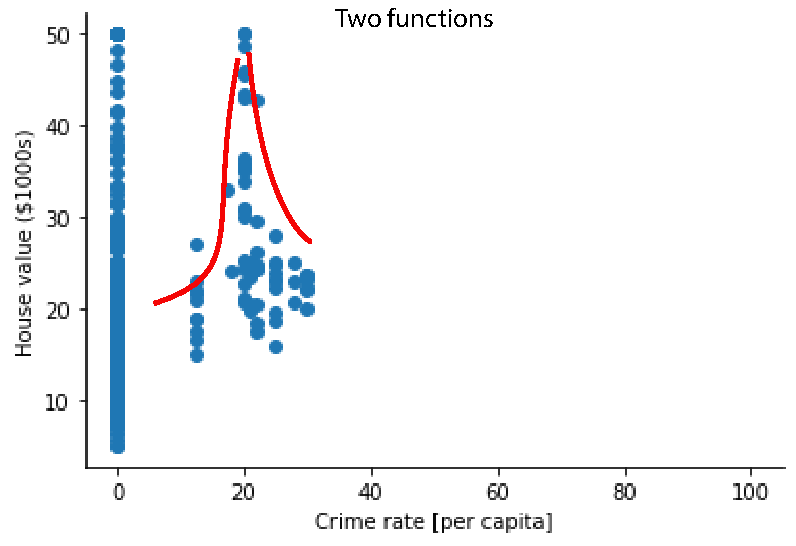
\includegraphics[scale=0.4]{boston_crimerate_lessdata.pdf}
      \hspace{6pt}}
    \uncover<3->{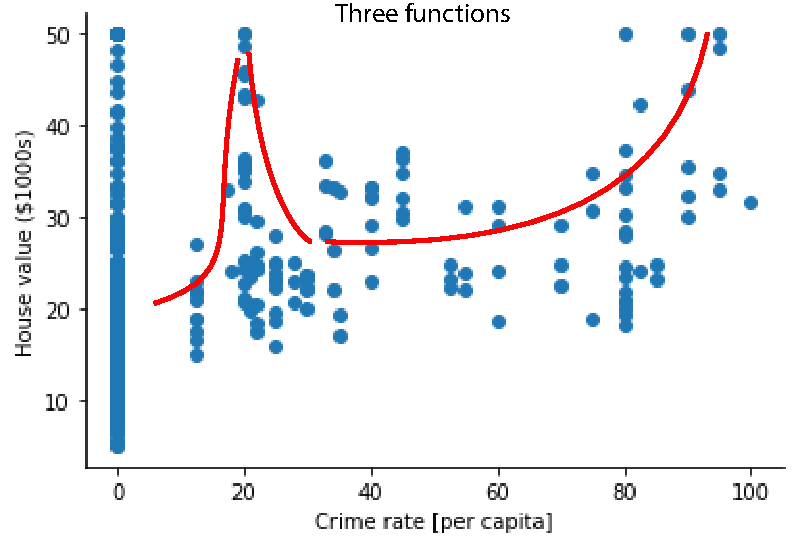
\includegraphics[scale=0.4]{boston_crimerate.pdf}}}

  % \centerline{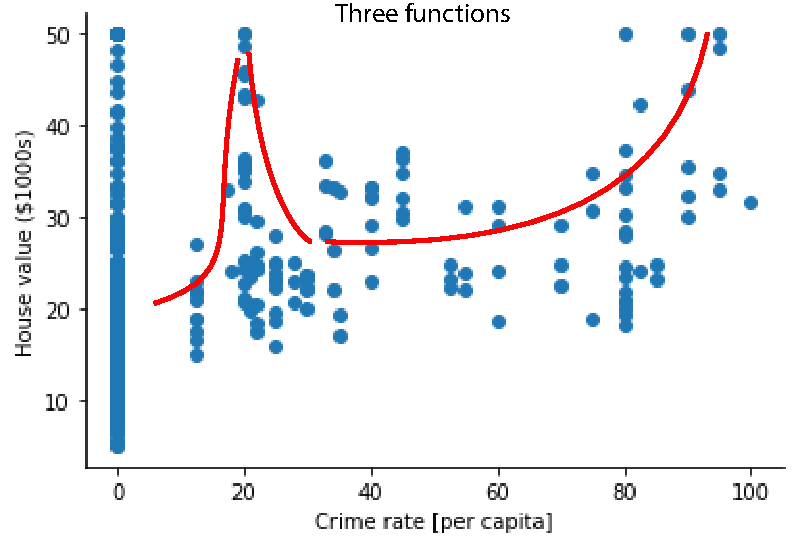
\includegraphics[scale=0.45]{boston_crimerate.png}}}
\end{frame}
%%%%%%%%%%%%%%%%%%%%%%%%%%%%%%%%%%%%%%%%%%%%%%%%%%%%%%%%%%%%%%%%%%%%%%

\begin{frame}[fragile]
\frametitle{Questions}

\begin{itemize}
\item Please also post questions on Teams or raise in the drop-in
  session or lab.
\vspace{12pt}

\uncover<2->{\item Quiz time! Go to Blackboard unit page $\gg$ Quizzes $\gg$ Lecture 1.  Should take you less than 3 minutes
\centerline{\includegraphics[scale=0.3]{BB.png}\vspace{10pt}}
}
\end{itemize}
\end{frame}



\end{document}
